\section{What comes next}
\label{sec:whatnext}

The results of this chapter describe the BDC process through its first and
second moments: the non-catastrophe and non-fixation probabilities, the mean
load, the mean release, and their variances, each in closed form and each
written as a function of the single quantity $I(t)$. Yet several of the
formulas we have derived hint at a richer structure that moments alone do not
capture. The ratio $V(t)/[1-I(t)]$ conditioned on rupture; the geometric form
of the burst size that surfaced in the $\mu=0$ check of
Theorem~\ref{thm:Wsq}; the finite plateau of the conditional mean $J/I$ in
\Figref{fig:J_of_t_1}'s neighbourhood --- each of these points beyond the
expectations, towards the full distributions of the process. Completing that
picture, and then embedding the single cell in a population, are the two
directions in which this thesis now moves.

% \figureflag{F3.5}{Burst-size preview}{%
% \textbf{Purpose:} preview the geometric burst-size law of Chapter~4a at the
% point where this chapter hands off to it, making the ``hint at richer
% structure'' in the text concrete. \textbf{Type:} Python analytic bar chart.
% \textbf{Content:} bars of $\Pr\{\Kb=k\}=(\delta/\lambda)a^{-k}$ for
% $(\lambda,\mu,\delta)=(1,0,0.1)$ and $k=1,\ldots,30$, where
% $a=(\lambda+\delta)/\lambda=1.1$ (the $\mu=0$ root); overlay the
% geometric$(1/a)$ probability mass function
% $\Pr\{k\}=(1-1/a)(1/a)^{k-1}$ as a connected curve to show the two coincide;
% annotate with a short text note that the mass at $\Kb=0$ is $b=0$ here (every
% realisation bursts when $\mu=0$), and that for $\mu>0$ the mass at zero would
% be $b$ and the non-zero sizes would keep the geometric ratio $1/a$.
% \textbf{Axes:} burst size $k$ (horizontal, 0--30), probability (vertical);
% legend entries ``$\Pr\{\Kb=k\}$'' and ``geometric$(1/a)$''. \textbf{Style:}
% unified Python style --- default matplotlib with \texttt{tab:} colours, grid
% alpha 0.25, \texttt{tight\_layout}, PDF output, fonts matching the chapter.
% \textbf{Data source:} the analytic law $\Pr\{\Kb=k\}=(\delta/\lambda)a^{-k}$
% (derived in Chapter~4a); no simulation. \textbf{Placement:}
% \Secref{sec:whatnext}, after the first paragraph.}

\begin{figure}[H]
\centering
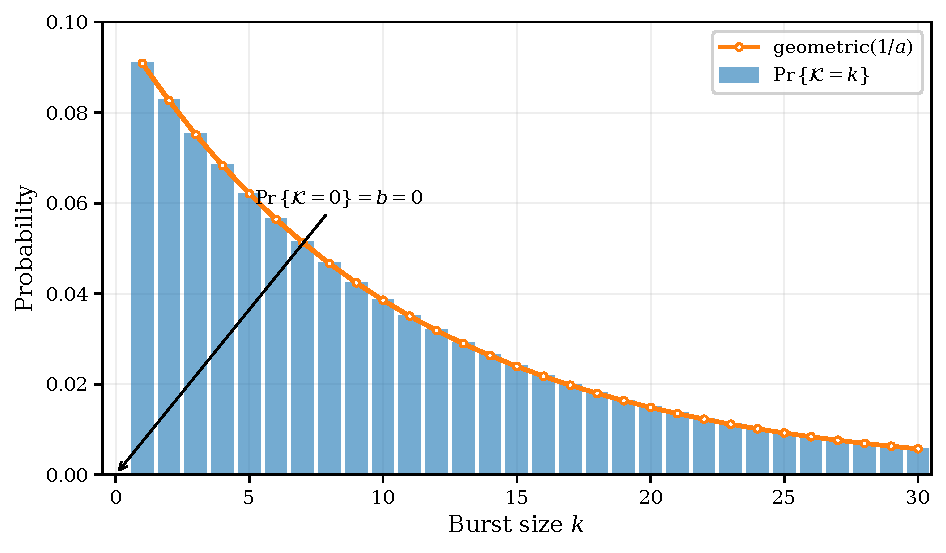
\includegraphics[width=0.72\textwidth]{figures/F3_5_burst_size_preview.pdf}
\caption{Burst-size preview for $\mu=0$: $\Pr\{\Kb=k\}=(\delta/\lambda)a^{-k}$
coincides with geometric$(1/a)$, while the mass at $\Kb=0$ is $b=0$.
Parameters $\lambda=1$, $\mu=0$, $\delta=0.1$, and $a=1.1$.}
\label{fig:F3_5_burst_size_preview}
\end{figure}

\subsection*{Completing the single-cell theory}

Chapter~4a completes the description of one infected cell. It solves the
probability generating function of the process and thereby obtains the state
probabilities $p_n(t)$ at every time --- not merely their sums $I$, $D$ and
$\Ifix$ --- and with them the quasi-stationary distribution: the limiting law
of the intracellular load conditioned on the cell remaining productive. The
burst time and burst size receive their full treatment there: the defective
density of $\tau$, the exact burst-size law $P_k=(\delta/\lambda)a^{-k}$ whose
$\mu=0$ preview appears above, and the conditional laws of burst size given
burst time and of burst time given burst size. The chapter also takes up the
multi-founder formulas of Section~\ref{sec:analytical}, which become essential
when a cell is infected by several particles at once, and it ends with the
chained immediate-transfer model, in which the released particles of one cell
found the next infection without delay. Everything in Chapter~4a rests on the
closed forms and identities of the present chapter, and nothing beyond them.

\subsection*{Embedding the cell in a population}

Chapter~4b turns from one cell to many. A released burst does not end the
story: the particles may go on to infect fresh cells, each starting its own
BDC trajectory. Modelling that population faithfully requires the
single-cell quantities of this chapter as \textit{age-dependent kernels} ---
the survival kernel $\Ifix(a)$, which says how many of the cells infected $a$
time units ago are still productive, and the release kernel $g(a)=\delta K(a)$,
which says when and how much they release. With these kernels the population
dynamics become a renewal system, and the constant-release ordinary
differential equations conventionally used in viral dynamics emerge only as an
approximation --- one that Chapter~4b shows to be quantitatively wrong in the
regimes that matter for early infection. The comparison between bursting and
its alternative, budding release, is taken up there as well.

Two open questions of the present chapter are answered by these developments:
the origin of the geometric burst-size law glimpsed in
Theorem~\ref{thm:Wsq}'s check (Chapter~4a derives it from the state
probabilities), and the status of the conditional plateau of $J/I$ (it is the
mean of the quasi-stationary distribution, and the burst size turns out to be
distributed exactly as that quasi-stationary law). What this chapter cannot
settle --- the evolutionary implications of releasing in one large burst
rather than continuously, and the behaviour of the population when released
particles compete for target cells --- is where the later chapters begin.
